% !TeX root = RJwrapper.tex
\title{A clustering algorithm to organize satellite hotspots data for the
purpose of tracking bushfires remotely}
\author{by Weihao Li, Emily Dodwell, and Dianne Cook}

\maketitle

\abstract{%
An abstract of less than 150 words.
}

\hypertarget{introduction}{%
\subsection{Introduction}\label{introduction}}

Bushfires are a major problem for Australia, and many other parts of the
globe. There is concern that as the climate becomes hotter, and drier,
that the impact of fires becomes much more severe and extensive. In
Australia, the 2019-2020 fires were the worst on record causing
extensive ecological damage, as well as damage to agricultural
resources, properties and infrastructure. The Wollemi pine, rare
prehistoric trees, required special forces intervention to prevent the
last stands in the world, in remote wilderness areas, from being turned
into ash.

Contributing to the problem is that many fires started in very remote
areas, locations deep into the temperate forests ignited by lightning,
that are virtually impossible to access or to monitor. Satellite data
provides a possible solution to this, particularly remotely sensed hot
spot data, which may be useful in detecting new ignitions and movements
of fires. Understanding fires in remote areas using satellite data may
provide some help in developing effective strategies for mitigating
bushfire impact.

This work addresses this topic. Using hot spot data, can we cluster in
space and time, in order to determine (1) points of ignition and (2)
track the movement of bush fires.

This paper is organised as follows. The next section provides an
introduction to the literature on spatiotemporal clustering and bush
fire modeling and dynamics. Section
\protect\hyperlink{algorithm}{Algorithm} describes the clustering
algorithm, and section \protect\hyperlink{application}{Application}
illustrates how the resulting data can be used to study bush fire
ignition.

\hypertarget{background}{%
\subsection{Background}\label{background}}

\hypertarget{spatiotemporal-clustering}{%
\subsubsection{Spatiotemporal
clustering}\label{spatiotemporal-clustering}}

\hypertarget{bushfire-modeling}{%
\subsubsection{Bushfire modeling}\label{bushfire-modeling}}

\hypertarget{algorithm}{%
\subsection{Algorithm}\label{algorithm}}

\hypertarget{data-pre-processing}{%
\subsubsection{Data pre-processing}\label{data-pre-processing}}

\begin{Schunk}
\begin{figure}
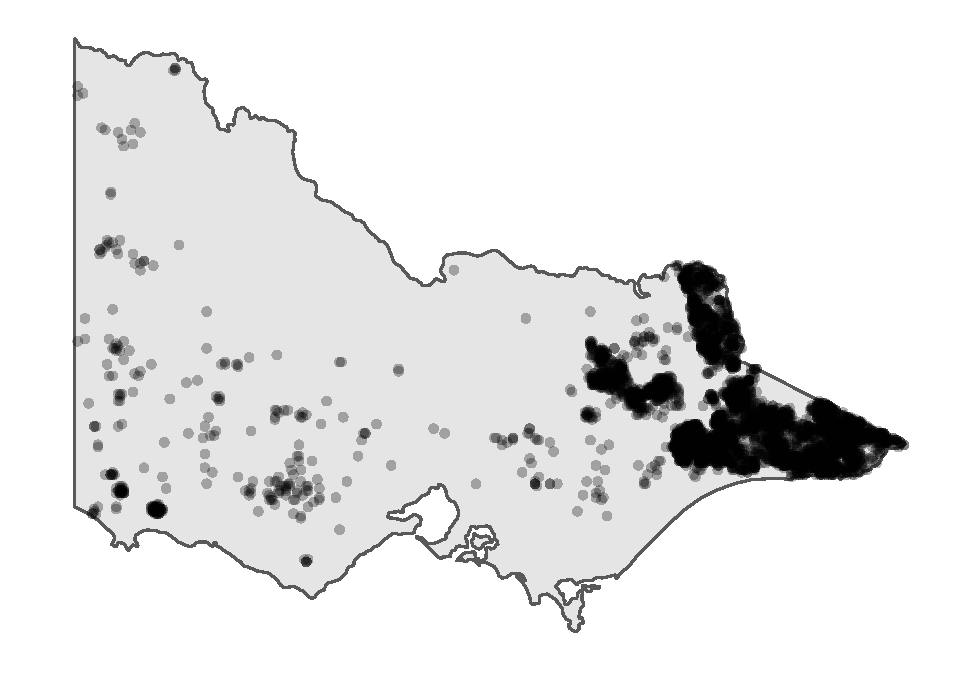
\includegraphics[width=0.8\linewidth]{clustering_paper_files/figure-latex/hotspots-1} \caption[Hotspot locations in Victoria during 2019-2020 season]{Hotspot locations in Victoria during 2019-2020 season.}\label{fig:hotspots}
\end{figure}
\end{Schunk}

\hypertarget{steps}{%
\subsubsection{Steps}\label{steps}}

This algorithm runs in a temporal manner. Starting from the first hour
of the first day or the bushfire season, hotspots are grouped, and then
agglomerated spatially. This proceeds to the next hour.

\textbf{1. Divide hotspots by hour}

Hostpots will first be divided into hours as shown in Figure
\ref{fig:step1}. Notice the unit of time is an arbitrary choice.
Theoretically, it can be replaced with any other units not larger than
the total length of time and not less than the temporal resolution of
the data. It depends on

\begin{Schunk}
\begin{figure}
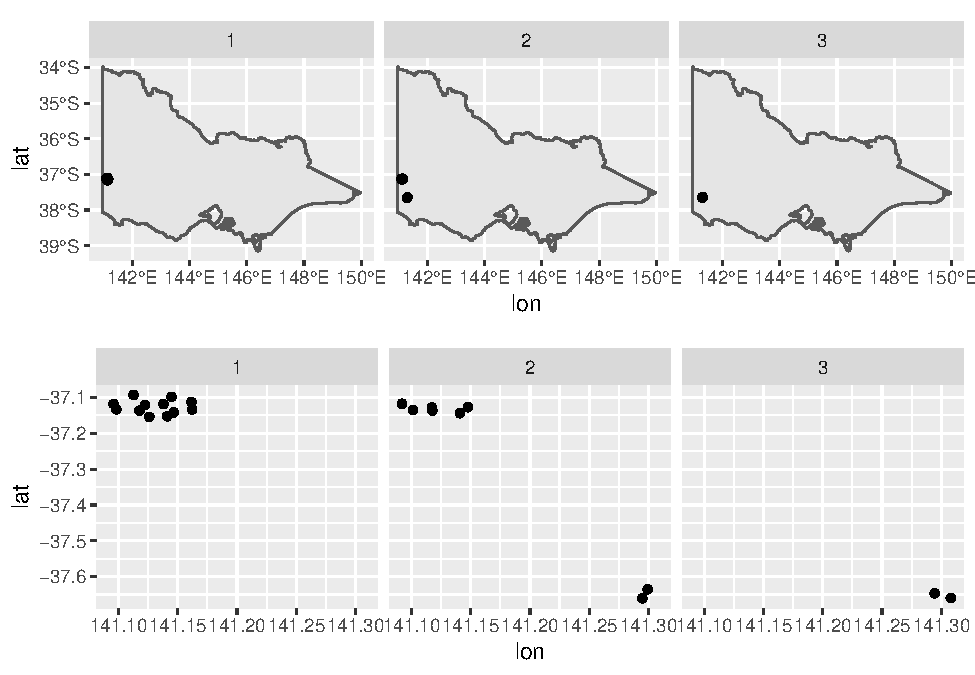
\includegraphics[width=0.8\linewidth]{clustering_paper_files/figure-latex/step1-1} \caption[Hotspots in the first 3 hours]{Hotspots in the first 3 hours.}\label{fig:step1}
\end{figure}
\end{Schunk}

\textbf{2. Start from the first hour}

Hotspots in the first hour will be filtered out from the data.

\begin{Schunk}

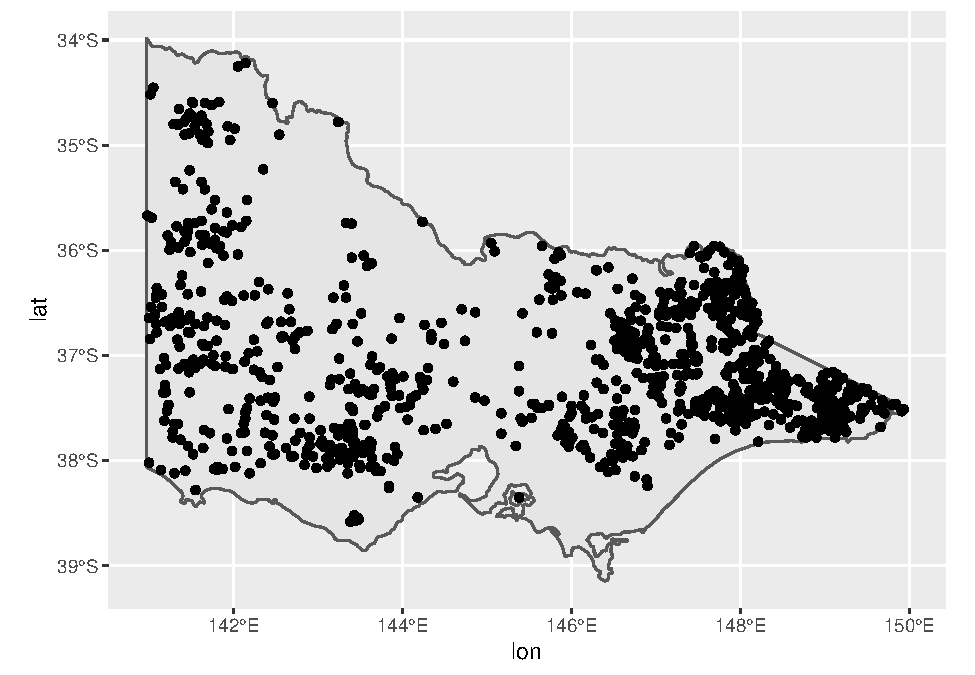
\includegraphics[width=0.8\linewidth]{clustering_paper_files/figure-latex/unnamed-chunk-2-1} \end{Schunk}

\textbf{3. Connect reachable hotspots}

We try to formalize the meaning of ``cluster'' to better illustrate the
connection between

\begin{defn}[directly reachable] A point p is directly reachable from a point q with respect to AdjDist, if the distance between point p and q is less or equal to AdjDist\end{defn}

\begin{defn}[reachable] A point p is reachable from a point q with respect to AdjDist, if there is a chain of points $p_1$, $p_2$, ..., $p_n$, $p_1 = p$, $P_n = q$ such that $P_n$ is directly reachable from $p_{n-1}$ \end{defn}

\hypertarget{effects-of-parameter-choices}{%
\subsubsection{Effects of parameter
choices}\label{effects-of-parameter-choices}}

There are two parameters that can be tuned in this algorithm. They are
\texttt{adj\_dist}, which is the density distance and
\texttt{active\_time}, which is the .

\hypertarget{application}{%
\subsection{Application}\label{application}}

\hypertarget{determining-the-ignition-point-and-time-for-individual-fires}{%
\subsubsection{Determining the ignition point and time for individual
fires}\label{determining-the-ignition-point-and-time-for-individual-fires}}

Show ignition points for a particularly heavy day and another for a
particularly light day

\begin{Schunk}

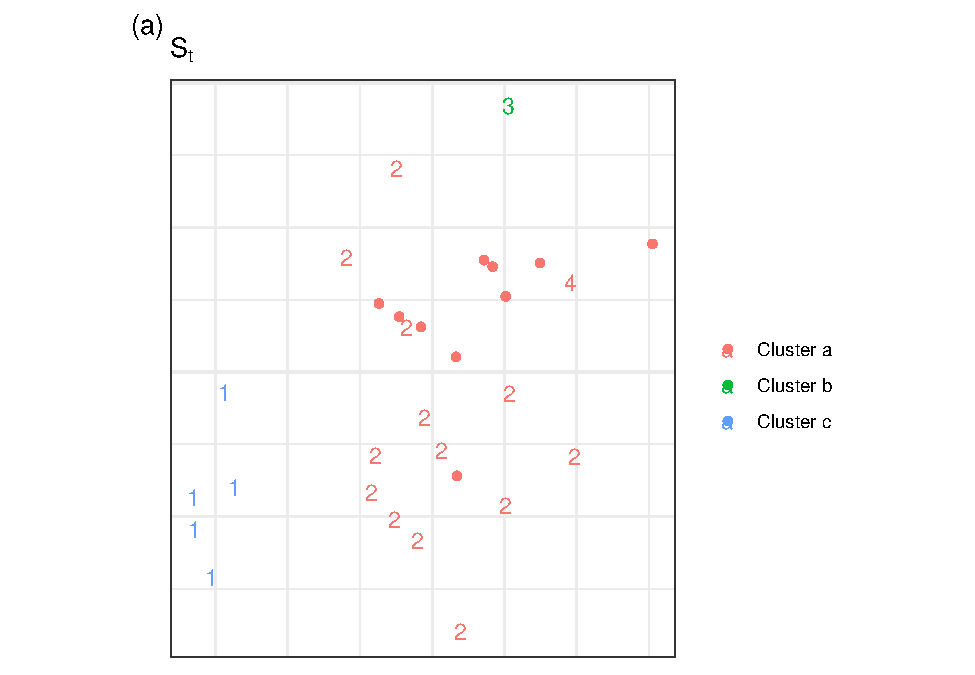
\includegraphics[width=0.8\linewidth]{clustering_paper_files/figure-latex/unnamed-chunk-3-1} \end{Schunk}

\begin{Schunk}

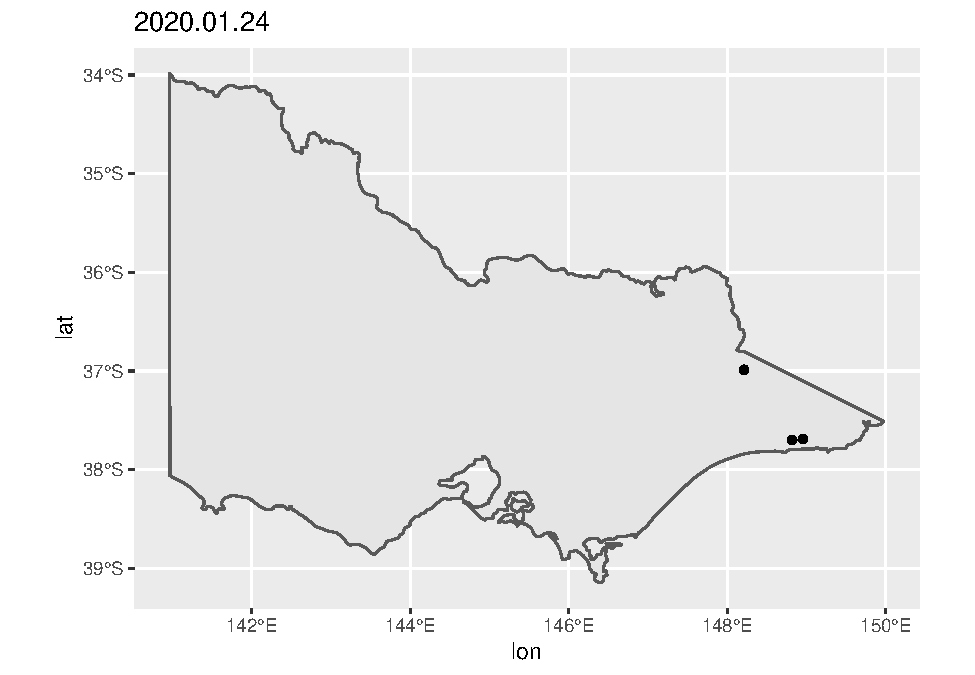
\includegraphics[width=0.8\linewidth]{clustering_paper_files/figure-latex/unnamed-chunk-5-1} \end{Schunk}

\begin{Schunk}

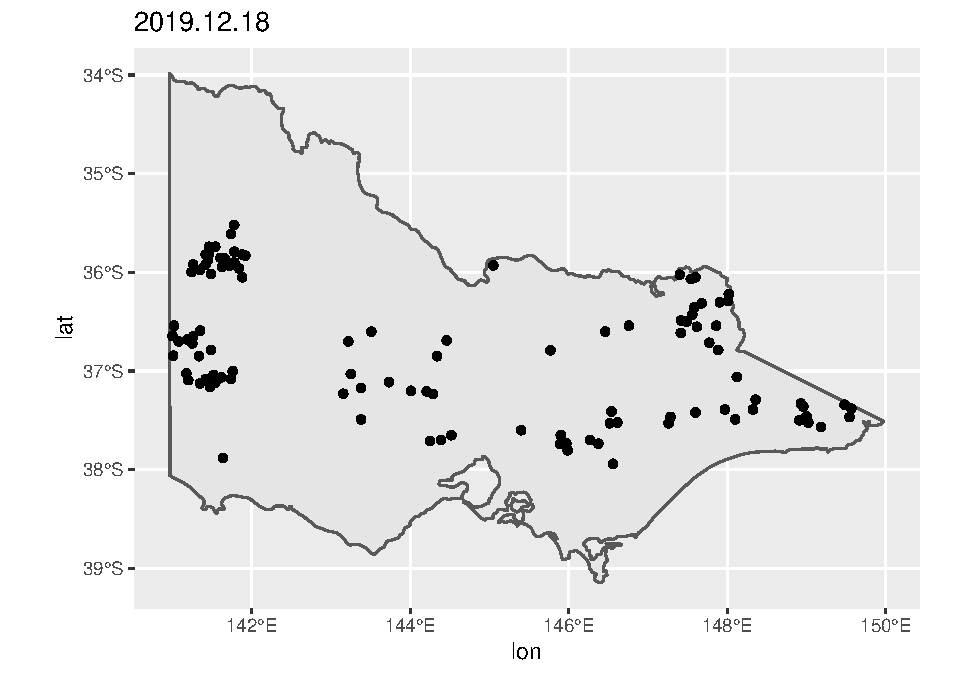
\includegraphics[width=0.8\linewidth]{clustering_paper_files/figure-latex/unnamed-chunk-6-1} \end{Schunk}

\hypertarget{tracking-fire-movement}{%
\subsubsection{Tracking fire movement}\label{tracking-fire-movement}}

Display showing how a fire moves over time, maybe two or more fires

\hypertarget{allocating-resources-for-future-fire-prevention}{%
\subsubsection{Allocating resources for future fire
prevention}\label{allocating-resources-for-future-fire-prevention}}

Merging data with camp sites, CFA, roads, \ldots{}

\hypertarget{summary}{%
\subsection{Summary}\label{summary}}

\hypertarget{acknowledgements}{%
\subsection{Acknowledgements}\label{acknowledgements}}

\begin{itemize}
\tightlist
\item
  The code and files to reproduce this work are at XXX
\item
  Data on hotspots can be downloaded from XXX
\end{itemize}

\bibliography{RJreferences}


\address{%
Weihao Li\\
Monash University\\%
line 1\\ line 2\\
%
%
%
\\\href{mailto:wlii0039@student.monash.edu}{\nolinkurl{wlii0039@student.monash.edu}}
}

\address{%
Emily Dodwell\\
AT\&T\\%
line 1\\ line 2\\
%
%
%
\\\href{mailto:emily@research.att.com}{\nolinkurl{emily@research.att.com}}
}

\address{%
Dianne Cook\\
Monash University\\%
line 1\\ line 2\\
%
%
%
\\\href{mailto:dicook@monash.edu}{\nolinkurl{dicook@monash.edu}}
}

